\documentclass[a4paper,12pt]{article} %Selecionando a classe que gera artigos.

%PACOTES ABNT
\usepackage[brazil]{babel} % Pacote para usar portugues.
%Babel traduz como “table of contents“, “chapter” e “section“, sejam impressas como “sumário”, “capítulo” e “seção”, respectivamente.

\usepackage[T1]{fontenc} %Pacote para copiar palavras com acentuação do pdf de um documento feito em LaTeX que tenha usado esses pacotes resultará nas palavras corretamente acentuadas

\usepackage[utf8]{inputenc} % Pacote para poder usar acentuação no arquivo .tex

%\usepackage{biblatex}


\usepackage{graphicx} %Pacote para inserir Figuras.

\usepackage[top=2.0cm,right=2.0cm,left=2.0cm,bottom=2.0cm]{geometry} %Pacote de Margens

\usepackage{enumerate} %Pacote para usar marcadores.

\usepackage[onehalfspacing]{setspace} %Pacote espaçamento 1,5 cm.

\usepackage[alf]{abntex2cite} % configura o sistema  de citações e referências para o estilo ABNT.


% alf = estilo autor-data, para citações.

%Para mais estilos de citações visite https://www.overleaf.com/learn/latex/Biblatex_bibliography_styles

%PACOTES ESSENCIAIS
\usepackage{graphicx,xcolor,comment,enumerate,multirow,multicol,indentfirst} %Pacote para inserir figuras, tabelas, editar cores das tabelas, numeração "Automática das figuras e tabelas", identar tabelas e figuras.


%PACOTES DE MATEMÁTICA
\usepackage{amsmath,amsthm,amsfonts,amssymb,dsfont,mathtools,blindtext} %Pacotes básicos de matemática.

\usepackage{sectsty}% http://ctan.org/pkg/sectsty
\usepackage{titlecaps}% http://ctan.org/pkg/titlecaps
\sectionfont{\normalsize\MakeUppercase}


\usepackage{fancyhdr}  % Para adicionar o rodapé
 %Pacotes principais

\fancypagestyle{empty}{%
\fancyhf{}% clear all header and footer fields
% \fancyfoot[L]{15º CONICT 2024} % except the center
\fancyfoot[C]{\thepage} % except the center
% \fancyfoot[R]{ISSN: 2178-9959} % except the center
\renewcommand{\headrulewidth}{0pt}%
\renewcommand{\footrulewidth}{0pt}%
}
\pagestyle{empty}

\begin{document} %Begin Inicia o Documento

%--------------------------------     NÃO ALTERAR    ----------------------------------------%
% Logo in the top right corner
\begin{flushright}
  
\includegraphics[width=4cm]{imagens/logo_ifsp_bri.png}
\end{flushright}

%-------------------------------------------------------------------------------------------------%



\begin{center}
%%%%%%%%%%%%%%%%%%%%%%%%%%%%%  ALTERAR TÍTULO, AUTORES  %%%%%%%%%%%%%%%%%%%%%%%%%%%%%%%%%%%%%%%%%%%%%

\vspace{0.5cm}
 \begin{center}
 \textbf{Ransomware: Um Estudo Abrangente sobre Ameaças, Estratégias de Defesa e Processos de Recuperação}
 \end{center}

\vspace{0.5cm}
José Augusto Cenci Castilho

%%%%%%%%%%%%%%%%%%%%%%%%%%%%%%%%%%%%%%%%%%%%%%%%%%%%%%%%%%%%%%%%%%%%%%%%%%%%%%%%%%%%%%%%%%%%%%%%%%%%%
%%%%%%%%%%%%%%%%%%%%%%%%%%%%INSERIR INFORMAÇÕES ALUNOS%%%%%%%%%%%%%%%%%%%%%%%%%%%%%%%%%%%%%%%%%
\begingroup
  \fontsize{9pt}{11pt}\selectfont
  
  Graduando em Engenharia de Computação, IFSP, Câmpus Birigui, j.cenci@aluno.ifsp.edu.br.

Área de conhecimento (Tabela CNPq): 1.03.03.04-9 Sistemas de Informação. 
\endgroup

%%%%%%%%%%%%%%%%%%%%%%%%%%%%%%%%%%%%%%%%%%%%%%%%%%%%%%%%%%%%%%%%%%%%%%%%%%%%%%%%%%%%%%%%%%%%%%%%
\end{center}
 %Alterar Título, autores, e apagar tabela !

%----------------------------------------TEXTOS-------------------------------------------------%


\vspace{0.5cm}
\noindent\textbf{RESUMO}: Nos dias de hoje o ransomware é como uma epidemia, que afeta as pessoas comuns e até as grandes empresas, 
onde os hackers solicitam pagamento para liberar dados infectados digitalmente.  


\vspace{0.5cm}
\noindent\textbf{PALAVRAS-CHAVE}: máximo de seis, separadas por ponto e vírgula (;), procurando não repetir palavras do 
título, escritas em letras minúsculas.. \cite{cloudflare_prevent}

\vspace{0.5cm}
\begin{center}
\textbf{TÍTULO EM INGLÊS}
\end{center}

\noindent\textbf{ABSTRACT}: Tradução do resumo para a língua inglesa.

\vspace{0.5cm}
\noindent\textbf{KEYWORDS}: Tradução das palavras-chave para a língua inglesa. %Resumo e Palavras-chave

% O que é
%  • Histórico
%  • Técnicas de ataque
%  • Os Ransomwares mais conhecidos – características
%  • Técnicas de proteção
%  • Como recuperar (quando é possível)

\section*{Introdução}

O ransomware emergiu como uma das ameaças cibernéticas mais proeminentes e disruptivas da atualidade, afetando organizações de todos os tamanhos 
e setores, bem como usuários individuais. Caracterizado pela sua capacidade de negar acesso a sistemas ou dados críticos, exigindo um resgate para a sua 
restauração, o ransomware não só causa perdas financeiras diretas, mas também interrupções operacionais significativas, danos à reputação e potenciais 
violações de dados sensíveis. A sua evolução constante, desde os primeiros exemplares rudimentares até às sofisticadas variantes atuais que empregam 
táticas de extorsão múltipla e modelos de negócio como Ransomware-as-a-Service (RaaS), sublinha a necessidade de uma compreensão aprofundada desta ameaça. 
Este artigo tem como objetivo fornecer uma análise abrangente do ransomware, abordando a sua definição, histórico evolutivo, as técnicas de ataque empregadas, 
as famílias mais notórias, as estratégias de proteção e as metodologias de recuperação, complementada por dados e tendências recentes.





 %Introdução

\section{O que é ransomware?}
Ransomware é uma categoria de software malicioso (malware) que impede ou limita o acesso dos usuários aos seus próprios 
sistemas ou arquivos pessoais. Para que o acesso seja restabelecido, os perpetradores exigem o pagamento de um resgate. 
De forma mais técnica, o ransomware é projetado para criptografar arquivos em um dispositivo, tornando quaisquer arquivos e os 
sistemas que dependem deles inutilizáveis. Os atores maliciosos então exigem um resgate em troca da chave de decriptografia. 
Frequentemente, esses atores também ameaçam vender ou vazar dados exfiltrados ou informações de autenticação caso o resgate não seja 
pago, uma tática conhecida como dupla extorsão.

Existem duas categorias principais de ransomware:
\begin{itemize}
    \item \textbf{Locker ransomware:} Este tipo bloqueia as funções básicas do computador, como o acesso ao desktop, e pode 
    desabilitar parcialmente o mouse e o teclado, permitindo interação apenas com a janela de exigência de resgate. 
    Geralmente, não visa arquivos críticos, mas sim bloquear o acesso.

    \item \textbf{Crypto ransomware:} Este tipo criptografa dados importantes como documentos, 
    imagens e vídeos, mas não interfere nas funções básicas do computador. Isso causa pânico, pois os usuários 
    podem ver seus arquivos, mas não acessá-los. Os desenvolvedores frequentemente incluem uma contagem regressiva, 
    ameaçando deletar todos os arquivos se o resgate não for pago dentro do prazo.
\end{itemize}

A Agência da União Europeia para a Cibersegurança (ENISA) define ransomware como um tipo 
de ataque onde os atores da ameaça tomam o controle dos ativos de um alvo e exigem um resgate em troca 
da devolução da disponibilidade do ativo ou em troca de não expor publicamente os dados do alvo. Esta definição 
abrange o cenário em evolução da ameaça, a prevalência de múltiplas técnicas de extorsão e os vários objetivos dos 
perpetradores, para além dos ganhos meramente financeiros. Desde o início de 2016, ocorreram, em média, mais de 4.000 
ataques de ransomware diariamente.

\section{Histórico do ransomware}
A história do ransomware, embora relativamente curta, demonstra uma evolução significativa em termos de sofisticação e impacto.   

\subsection{O Pioneiro: AIDS Trojan (PC Cyborg)}
O primeiro caso documentado de ransomware remonta a dezembro de 1989, com o surgimento do AIDS Trojan, 
também conhecido como PC Cyborg. Criado pelo Dr. Joseph Popp, um biólogo educado em Harvard, este malware foi distribuído 
através de aproximadamente 20.000 disquetes enviados pelo correio para pesquisadores da AIDS e assinantes de revistas científicas 
em cerca de 90 países. O malware não criptografava o conteúdo dos arquivos, mas sim os nomes dos arquivos e ocultava diretórios no 
disco C: após o sistema ser reiniciado 90 vezes. Uma nota de resgate exigia o pagamento de \$189 ou \$378 para uma caixa postal no 
Panamá para "renovar a licença" do software. 

Embora rudimentar pelos padrões atuais – escrito em QUICKBASIC 3.0 e utilizando uma cifra de substituição simétrica 
simples nos nomes dos arquivos – o AIDS Trojan estabeleceu o precedente para a extorsão digital. Ferramentas de remoção e 
decriptografia (AIDSOUT, AIDSCLEAR e CLEARAID) foram rapidamente desenvolvidas por Jim Bates e John Sutcliffe. 
O Dr. Popp foi preso, mas nunca cumpriu pena, e acredita-se que suas ações foram um catalisador para a criação do 
Computer Misuse Act de 1990 no Reino Unido, país escolhido para a distribuição dos disquetes devido à ausência de leis específicas 
contra o uso indevido de computadores na época. Este primeiro ransomware, apesar de sua simplicidade e do alto custo de distribuição, 
demonstrou o potencial de dano e lançou as bases conceituais para futuras táticas de extorsão cibernética, mesmo que sua 
execução técnica fosse primitiva e o impacto financeiro para o perpetrador, insignificante. 
A tentativa de extorsão foi dificultada pelo uso limitado de computadores na época.


\subsection{Evolução e Sofisticação}

Após o AIDS Trojan, o cenário de ransomware permaneceu relativamente quiescente até meados dos anos 2000, quando os criminosos 
cibernéticos começaram a experimentar métodos de criptografia mais robustos e mecanismos de pagamento anônimos.

Primeiros Lockers e Scareware (Meados dos anos 2000 - Início dos anos 2010): Surgiram os ransomware lockers, 
que bloqueavam o acesso ao sistema operacional ou a arquivos essenciais, e o scareware, que exibia falsos alertas de infecção por 
vírus, exigindo pagamento para "limpeza". Em 2006-2007, variantes como o GPCode utilizavam criptografia simétrica falha, 
mas versões posteriores empregaram métodos mais fortes e chaves mais longas (1024 ou 2048 bits), dificultando a recuperação.

A Era da Criptografia Forte e Criptomoedas (A partir de 2013): O ano de 2013 marcou um ponto de inflexão com o 
surgimento do CryptoLocker. Este foi um dos primeiros a utilizar criptografia assimétrica forte (RSA-2048) para tornar os 
arquivos inacessíveis e exigia pagamento em Bitcoin, garantindo maior anonimato aos criminosos. 
O CryptoLocker se disseminava principalmente por meio de e-mails de phishing com anexos maliciosos e, até o final de 2015, 
teria rendido aos seus operadores cerca de \$27 milhões. Este sucesso financeiro demonstrou a lucratividade do modelo e 
impulsionou o desenvolvimento de novas famílias de ransomware.

Ransomware-as-a-Service (RaaS) e Dupla Extorsão (Final dos anos 2010 - Presente): O modelo de Ransomware-as-a-Service (RaaS) 
democratizou o acesso a ferramentas de ransomware, permitindo que indivíduos com menos conhecimento técnico lançassem ataques 
em troca de uma porcentagem do resgate pago pelas vítimas. Isso levou a um aumento exponencial no volume de ataques. 
Em 2020, o custo global do ransomware atingiu \$20 bilhões.
A tática de dupla extorsão, popularizada pelo grupo Maze em 2020, adicionou uma nova camada de 
pressão: além de criptografar os dados, os atacantes os exfiltram e ameaçam publicá-los caso o resgate não seja pago. 
Esta abordagem torna os backups, por si só, insuficientes para mitigar completamente o risco, pois não impedem a exposição 
de dados sensíveis. Dados da BlackFog para 2024 indicam que mais de 93\% dos ataques de ransomware incluem um elemento de 
exfiltração de dados.


\begin{table}[htbp]
    \centering
    \small
    \caption{Evolução Histórica do Ransomware}
    \label{tab:evolucao_historica}
    % \sloppy
    \begin{tabularx}{\textwidth}{|l|p{3cm}|p{5cm}|p{5cm}|}
        \hline
        \textbf{Período} & \textbf{Marco Principal} & \textbf{Características Notáveis} & \textbf{Impacto Significativo} \\ \hline
        1989 & AIDS Trojan (PC Cyborg) & Distribuição via disquetes, ocultação de diretórios, nomes de arquivos criptografados 
        (simples), resgate por correio postal. & Primeiro ransomware documentado; catalisador para leis de crimes cibernéticos. 
        \cite{CyberMaxxRansomwareHistory, Muniandy2024Ransomware, WatchGuardAIDSTrojan} \\ \hline
        Meados dos anos 2000 & Surgimento de \textit{Lockers} e \textit{Scareware} & Bloqueio de tela/sistema; falsos alertas de vírus; 
        criptografia simétrica fraca (e.g., GPCode). & Aumento gradual da atividade; experimentação com modelos de extorsão. 
        \cite{Tanni2022RedAlert, MasterDCRansomwareHowItWorks, Robb2024RansomwareHistory} \\ \hline
        2013 & CryptoLocker & Criptografia assimétrica forte (RSA); uso de Bitcoin para pagamento; disseminação via 
        \textit{phishing}. & Revolucionou o ransomware, tornando a recuperação quase impossível sem a chave; alta lucratividade. 
        \cite{CyberMaxxRansomwareHistory, Muniandy2024Ransomware, Robb2024RansomwareHistory} \\ \hline
        Fim de 2010 & Ascensão do \textit{Ransomware-as-a-Service} (RaaS) & Plataformas oferecem ransomware a afiliados; 
        divisão de lucros; proliferação de ataques. & Redução da barreira de entrada para cibercriminosos; aumento massivo no 
        volume de ataques. \cite{CyberMaxxRansomwareHistory, Robb2024RansomwareHistory} \\ \hline
        2017 & WannaCry & Exploração da vulnerabilidade EternalBlue (SMB); propagação tipo \textit{worm}; impacto global em 
        larga escala. & Demonstrou a capacidade de interrupção massiva e a vulnerabilidade de sistemas não corrigidos. 
        \cite{CyberMaxxRansomwareHistory, WikipediaWannaCry} \\ \hline
        2020 & Predominância da Dupla e Tripla Extorsão & Exfiltração de dados antes da criptografia; ameaça 
        de vazamento público; ataques DDoS adicionais. & Aumenta a pressão sobre as vítimas; \textit{backups} sozinhos não 
        são suficientes. \cite{CyberMaxxRansomwareHistory, Robb2024RansomwareHistory, ThreatDownALPHVBlackCat, AkamaiBlackCatRansomware} \\ \hline
        2021 & Foco em Alvos de Alto Valor e Infraestruturas Críticas & Ataques direcionados a grandes 
        corporações, hospitais, governos; demandas de resgate milionárias. & Interrupções severas em serviços essenciais; 
        aumento do impacto econômico e social. \cite{CyberMaxxRansomwareHistory, Robb2024RansomwareHistory} \\ \hline
        2023 & Uso Crescente de IA e Exploração de Novas Vulnerabilidades & Desenvolvimento de ransomware assistido 
        por IA; exploração de vulnerabilidades em dispositivos IoT e \textit{firmware}. & Potencial para ataques mais sofisticados, 
        evasivos e automatizados. \cite{ENISA_ETL_2023, KasperskyRansomwareReport2025} \\ \hline
    \end{tabularx}
\end{table}

A sofisticação crescente dos ataques e a profissionalização dos grupos de ransomware, evidenciada 
por vazamentos como os do grupo Conti em 2022, que revelaram suas ferramentas internas, guias de ataque e 
estruturas operacionais, demonstram a natureza empresarial dessas operações criminosas. A adaptação contínua dos 
criminosos, como o desenvolvimento de variantes para sistemas Linux e ESXi, visa ampliar a superfície de ataque e maximizar o 
impacto e as demandas de resgate.

\section{Técnicas de ataque}

Os ataques de ransomware envolvem um ciclo de vida com múltiplas fases, desde a penetração inicial 
até a extorsão. Compreender as técnicas empregadas em cada fase é crucial para desenvolver defesas eficazes.

\subsection{Vetores de Infecção Comuns}

Os atores de ransomware utilizam diversos vetores para obter acesso inicial aos sistemas das vítimas:

\begin{itemize}
    \item \textbf{E-mails de Phishing e Spear-Phishing:} Continuam sendo os vetores mais comuns. E-mails fraudulentos, muitas 
    vezes com um senso de urgência ou disfarçados de comunicações legítimas, contêm links maliciosos ou anexos infectados 
    (e.g., documentos PDF, ZIP, Microsoft Office com macros). Ao clicar no link ou abrir o anexo, o usuário pode ser redirecionado 
    para sites falsos que baixam o ransomware ou exploit kits. A ENISA aponta que o phishing permanece como o principal vetor de 
    infecção inicial, especialmente na região EMEA (40\% das violações).
    
    \item \textbf{Exploração de Vulnerabilidades em Software:} Sistemas e softwares desatualizados ou não corrigidos são alvos 
    frequentes. Os atacantes exploram vulnerabilidades conhecidas (CVEs) em aplicações voltadas para a internet, como servidores web, 
    VPNs e protocolos de desktop remoto. O relatório da Unit 42 de 2022 indicou que 48\% dos casos de ransomware começaram com 
    vulnerabilidades de software. A exploração da vulnerabilidade CVE-2023-0669 no software GoAnywhere MFT pela Cl0p resultou em um 
    aumento nos ataques em março de 2023.
    
    \item \textbf{Protocolo de Desktop Remoto (RDP) e Outros Serviços Remotos Mal Configurados:} Credenciais RDP fracas ou expostas 
    são um alvo comum para ataques de força bruta ou compra em mercados clandestinos. Uma vez obtido o acesso RDP, os atacantes podem 
    implantar o ransomware diretamente.
    
    \item \textbf{Malvertising e Drive-by Downloads:} Anúncios maliciosos em sites legítimos ou comprometidos podem redirecionar 
    usuários para sites que hospedam exploit kits ou iniciam o download automático de ransomware sem a interação do usuário.
    
    \item \textbf{Credenciais Comprometidas:} O uso de credenciais roubadas (obtidas através de violações de dados anteriores, 
    infostealers ou phishing) permite que os atacantes acessem sistemas como usuários legítimos, contornando algumas defesas. 
    O relatório DBIR 2025 da Verizon destaca que o abuso de credenciais (22\%) é um dos principais vetores de ataque inicial.
    
    \item \textbf{Ataques à Cadeia de Suprimentos:} Comprometimento de fornecedores de software ou provedores de serviços 
    gerenciados (MSPs) para distribuir ransomware aos seus clientes, como no ataque à Kaseya pelo REvil.
    
    \item \textbf{Dispositivos USB Infectados:} Embora menos comum para ataques em larga escala, o uso de dispositivos USB 
    infectados ainda pode ser um vetor, especialmente em ambientes com controles de segurança física deficientes.
\end{itemize}

Relatórios recentes da ENISA (2023) indicam uma mudança, com links URL e navegação na web 
emergindo como métodos dominantes para entrega de ransomware, respondendo por mais de 77\% dos casos, superando os anexos de e-mail.

\subsection{Fases do Ataque Após a Infecção Inicial}

Uma vez que o acesso inicial é obtido, o ataque de ransomware normalmente progride através das seguintes fases \cite{MasterDCRansomwareHowItWorks, ResearchGateRansomwareInfectionVector, Casino2025RansomwareDetection}:

\begin{enumerate}
    \item \textbf{Reconhecimento e Movimentação Lateral}: O atacante explora a rede para identificar ativos críticos, dados 
    valiosos e sistemas adicionais para comprometer \cite{MasterDCRansomwareHowItWorks, ThreatDownALPHVBlackCat, 
    ResearchGateRansomwareInfectionVector, Casino2025RansomwareDetection}. Ferramentas como \texttt{Mimikatz} podem 
    ser usadas para extrair credenciais e escalar privilégios \cite{WikipediaLockBit}. A movimentação lateral visa expandir 
    o controle sobre a rede da vítima.

    \item \textbf{Exfiltração de Dados (Dupla Extorsão)}: Antes da criptografia, os atacantes frequentemente 
    exfiltram grandes volumes de dados sensíveis para servidores sob seu controle 
    \cite{CyberMaxxRansomwareHistory, Robb2024RansomwareHistory, ThreatDownALPHVBlackCat, MandiantGoogleCloudRansomware2023}. 
    Ferramentas comuns de exfiltração incluem \texttt{Rclone}, \texttt{MEGASync}, \texttt{FileZilla} e \texttt{WinSCP}, além de 
    ferramentas personalizadas como \texttt{EXMATTER} e \texttt{EXBYTE} \cite{MandiantGoogleCloudRansomware2023}. 
    Esta etapa é fundamental para a tática de dupla extorsão.

    \item \textbf{Criptografia de Dados}: Esta é a fase central do ataque de \textit{crypto ransomware}. 
    O \textit{malware} procura e criptografa arquivos com extensões específicas (e.g., \texttt{.doc}, \texttt{.jpg}, 
    \texttt{.pdf}, bancos de dados) \cite{Tanni2022RedAlert}. Algoritmos de criptografia fortes são empregados:
    \begin{itemize}
        \item \textbf{Criptografia Simétrica}: Utiliza uma única chave tanto para criptografar quanto para decriptografar os dados. 
        É rápida, mas a chave precisa ser distribuída ou armazenada no \textit{malware}, tornando-a vulnerável à engenharia reversa 
        se não for protegida adequadamente \cite{Tanni2022RedAlert}.
        \item \textbf{Criptografia Assimétrica (Chave Pública)}: Utiliza um par de chaves: uma pública para criptografar e 
        uma privada para decriptografar. A chave pública pode ser distribuída abertamente, enquanto a chave privada é mantida em 
        segredo pelo atacante. É mais lenta que a simétrica para grandes volumes de dados \cite{Tanni2022RedAlert}.
        \item \textbf{Criptografia Híbrida}: Combina a eficiência da criptografia simétrica com a segurança da assimétrica. 
        Tipicamente, o ransomware gera uma chave simétrica aleatória para cada arquivo (ou um conjunto de arquivos), criptografa 
        os dados com essa chave simétrica, e então criptografa a chave simétrica com a chave pública do atacante. A chave privada 
        do atacante, necessária para decriptografar a chave simétrica (e, por conseguinte, os arquivos), é mantida no servidor de 
        Comando e Controle (C2) \cite{Tanni2022RedAlert}. Este é o método mais comum e robusto.
    \end{itemize}
    O ransomware pode chamar APIs criptográficas do sistema operacional da vítima para gerar chaves \cite{Tanni2022RedAlert}. 
    Algumas variantes, como o Ryuk, incorporam chaves públicas RSA (e.g., RSA-2048) e usam AES-256 para a criptografia de arquivos 
    \cite{CrowdStrikeRyukAnalysis}. O objetivo é tornar a recuperação sem a chave privada do atacante computacionalmente inviável.

    \item \textbf{Comunicação com Servidor de Comando e Controle (C2)}: Muitos ransomwares se comunicam com servidores C2 
    para enviar informações da vítima, baixar módulos adicionais, e, crucialmente, obter ou enviar chaves de criptografia 
    \cite{Tanni2022RedAlert}. A chave simétrica usada para criptografar os arquivos da vítima é frequentemente criptografada 
    com a chave pública do C2, e a chave privada correspondente permanece com os atacantes \cite{Tanni2022RedAlert}.

    \item \textbf{Exibição da Nota de Resgate e Exigência de Pagamento}: Após a criptografia, uma nota de resgate é 
    exibida na tela da vítima ou em arquivos de texto (\texttt{.txt}, \texttt{.html}) deixados nos diretórios afetados 
    \cite{Muniandy2024Ransomware, WikipediaLockBit}. A nota instrui a vítima sobre como pagar o resgate (geralmente em 
    criptomoedas como Bitcoin ou Monero devido ao seu pseudo-anonimato) para obter a ferramenta de decriptografia 
    \cite{Tanni2022RedAlert, CyberMaxxRansomwareHistory}. As notas podem incluir ameaças de aumento do valor do resgate 
    com o tempo ou de publicação dos dados exfiltrados \cite{WikipediaWannaCry}.
\end{enumerate}

A detecção precoce e o bloqueio do processo de criptografia são cruciais. 
Abordagens de detecção podem monitorar eventos de escrita no sistema de arquivos, 
procurando por arquivos com alta entropia (característica de dados criptografados ou comprimidos), 
embora diferenciar entre os dois possa ser um desafio \cite{Casino2025RansomwareDetection}.

\section{Os ransomwares mais conhecidos}

Diversas famílias de ransomware ganharam notoriedade devido ao seu impacto, sofisticação ou volume de ataques. Abaixo, detalhamos algumas das mais conhecidas:

\subsection{LockBit}
\textbf{Modelo e Operação:} LockBit é um grupo cibercriminoso que opera um proeminente modelo de Ransomware-as-a-Service (RaaS) desde sua aparição em fóruns de cibercrime de língua russa em janeiro de 2020. Ele recruta afiliados para conduzir ataques, utilizando táticas de dupla extorsão: criptografia de dados e ameaça de vazamento público.

\textbf{Evolução:} Conhecido anteriormente como ".abcd" (devido à extensão de arquivo adicionada aos arquivos criptografados), evoluiu para LockBit 2.0 em 2021 e LockBit 3.0 (ou LockBit Black) em março de 2022, com recursos aprimorados e criptografia mais robusta. Em janeiro de 2023, foi lançado o LockBit Green, incorporando código do ransomware Conti.

\textbf{Técnicas:} O LockBit se auto-propaga dentro de uma rede usando Windows PowerShell e Server Message Block (SMB). Utiliza ferramentas como Mimikatz para coletar credenciais, desabilita produtos de segurança e evade defesas. A criptografia é realizada com AES e RSA, criptografando apenas os primeiros kilobytes de cada arquivo para maior velocidade e adicionando a extensão ".lockbit". Notas de resgate são exibidas como papel de parede e podem ser impressas.

\textbf{Alvos e Impacto:} O LockBit foi o ransomware mais prolífico em 2022, responsável por 44\% de todos os incidentes de ransomware globalmente no início de 2023. Entre janeiro de 2020 e maio de 2023, foi usado em aproximadamente 1.700 ataques nos EUA, resultando em \$91 milhões pagos em resgates. Alvos notáveis incluem Accenture (julho de 2021), Thales (janeiro de 2022), o hospital de Corbeil Essonnes na França (setembro de 2022, resgate de \$10 milhões), e o Hospital for Sick Children de Toronto (dezembro de 2022), onde o grupo pediu desculpas e ofereceu a solução de decriptografia gratuitamente, alegando uma política contra atacar hospitais.

\textbf{Status Atual:} Em fevereiro de 2024, agências de aplicação da lei apreenderam o controle dos sites da dark web do LockBit. Apesar das ações policiais, variantes e afiliados podem continuar ativos.

\subsection{Conti}
\textbf{Modelo e Operação:} Conti foi um grupo de RaaS altamente ativo entre dezembro de 2019 e maio de 2022, acreditado ser operado pelo grupo russo Wizard Spider e possivelmente evoluído do Ryuk. Os desenvolvedores alugavam seu malware para afiliados, que realizavam os ataques e dividiam os lucros.

\textbf{Técnicas:} Conti utilizava diversas técnicas de infecção, incluindo e-mails de phishing (com malware BazarLoader), exploração de vulnerabilidades de software (como no protocolo SMB), e o uso de outros malwares como o TrickBot e ferramentas legítimas de simulação de adversário como Cobalt Strike. Após o acesso inicial, desabilitava ferramentas de segurança, movia-se lateralmente, exfiltrava dados valiosos e utilizava criptografia multi-threaded para rápida encriptação de arquivos, podendo também deletar backups. Empregava táticas de dupla extorsão, com um site de vazamento para publicar dados roubados.

\textbf{Alvos e Impacto:} Conti era conhecido por ataques agressivos a uma vasta gama de organizações públicas e privadas, incluindo saúde, educação, governos e infraestruturas críticas. Ataques notáveis incluem JVCKenwood (setembro de 2021), o Health Service Executive (HSE) da Irlanda (maio de 2021, forçando o desligamento do sistema), o governo da Costa Rica (abril de 2022, levando à declaração de emergência nacional) e a cidade de Tulsa (maio de 2021).

\textbf{Status Atual:} O grupo sofreu um grande golpe em fevereiro de 2022, quando declarou apoio à invasão da Ucrânia pela Rússia, o que reduziu sua receita, pois as vítimas se tornaram relutantes em pagar. Concomitantemente, um insider vazou conversas internas e código-fonte, expondo as operações do grupo. Embora o Conti tenha encerrado seu site e ataques sob essa marca em 2022, acredita-se que seus membros se reorganizaram em outras operações de ransomware.

\subsection{Ryuk}
\textbf{Origem e Operação:} Ryuk surgiu em agosto de 2018, sendo operado pelo sofisticado grupo de eCrime WIZARD SPIDER. É derivado do código-fonte do Hermes, um ransomware comercial, mas Ryuk foi especificamente adaptado para ataques direcionados a grandes organizações ("big game hunting") em busca de resgates elevados.

\textbf{Técnicas:} Ryuk é conhecido por sua capacidade de identificar e criptografar unidades de rede e recursos, além de deletar cópias de sombra (shadow copies) no endpoint, impossibilitando a restauração do sistema Windows sem backups externos. A criptografia utiliza RSA-2048 e AES-256, com chaves armazenadas no executável no formato Microsoft SIMPLEBLOB e um marcador de arquivo "HERMES". Uma diferença notável em relação ao Hermes é que o Ryuk incorpora duas chaves RSA públicas no executável e não gera um par de chaves RSA específico da vítima no host; em vez disso, a chave privada da "vítima" (usada para proteger a chave AES de criptografia de arquivo) é também criptografada e embutida, sugerindo que pares de chaves RSA são pré-gerados para cada vítima/executável. A entrega frequentemente ocorre após infecções pelos trojans Emotet e TrickBot, que fornecem o acesso inicial e as credenciais administrativas.

\textbf{Alvos e Impacto:} Ryuk visa organizações de alto perfil onde os atacantes esperam pagamentos significativos, como EMCOR, hospitais UHS e diversos jornais. Estima-se que tenha gerado \$61 milhões para seus operadores entre fevereiro de 2018 e outubro de 2019. O valor do resgate varia consideravelmente, sugerindo um cálculo baseado no tamanho e valor da organização vítima.

\textbf{Status Atual:} Embora grupos como WIZARD SPIDER possam adaptar suas ferramentas, o Ryuk como marca específica pode ter sido sucedido por outras variantes ou operações do mesmo grupo.

\subsection{WannaCry}
\textbf{Origem e Propagação:} O ataque WannaCry em maio de 2017 foi um evento global que explorou a vulnerabilidade EternalBlue no protocolo SMB do Microsoft Windows. O EternalBlue, um exploit desenvolvido pela NSA dos EUA, foi vazado pelo grupo The Shadow Brokers um mês antes do ataque. WannaCry agia como um cryptoworm, espalhando-se automaticamente para computadores vulneráveis na mesma rede e aleatoriamente pela Internet.

\textbf{Técnicas:} Ao ser executado, verificava um "kill switch" (um nome de domínio específico); se não encontrado, criptografava os dados do computador e tentava se propagar. Utilizava a ferramenta DoublePulsar para instalar e executar cópias de si mesmo. Exigia resgate em Bitcoin, cerca de US\$300 a US\$600.

\textbf{Impacto:} Infectou mais de 230.000 computadores em mais de 150 países em um dia. Organizações que não haviam aplicado o patch de segurança da Microsoft de março de 2017 foram afetadas, com um impacto particularmente severo em sistemas Windows não suportados como o XP (embora estudos da Kaspersky Lab tenham indicado que 98\% dos computadores afetados rodavam Windows 7). O Serviço Nacional de Saúde (NHS) do Reino Unido foi um dos mais atingidos, com até 70.000 dispositivos afetados e um custo de recuperação de \$100 milhões. As perdas econômicas globais foram estimadas em mais de \$4 bilhões. O ataque foi interrompido algumas horas após seu início pela descoberta e registro do domínio kill switch por Marcus Hutchins.

\textbf{Status Atual:} Embora o WannaCry original tenha sido contido, a vulnerabilidade EternalBlue continuou a ser explorada por outros malwares, e variantes do WannaCry podem ter surgido.

\subsection{CryptoLocker}
\textbf{Contexto Histórico:} Surgiu em setembro de 2013 e operou principalmente até maio de 2014. Foi um dos primeiros ransomwares a usar criptografia assimétrica forte (RSA-2048) de forma eficaz e a exigir pagamento em Bitcoin.

\textbf{Técnicas:} Disseminava-se através de anexos de e-mail infectados (frequentemente arquivos ZIP disfarçados de notificações de empresas de logística ou faturas). Após a infecção, buscava e criptografava arquivos com extensões comuns (documentos, imagens). As chaves de decriptografia eram armazenadas nos servidores dos atacantes.

\textbf{Impacto:} Estima-se que tenha infectado cerca de 500.000 máquinas. A operação foi significativamente desmantelada pela Operação Tovar, que derrubou a botnet Gameover ZeuS, usada para distribuir o CryptoLocker. Um portal online foi criado por autoridades e empresas de segurança para que as vítimas pudessem obter chaves de decriptografia gratuitamente, após a apreensão de parte da infraestrutura dos criminosos.

\textbf{Status Atual:} Inativo, mas seu sucesso pavimentou o caminho para muitos outros crypto ransomwares.

\subsection{REvil (Sodinokibi)}
\textbf{Modelo e Operação:} REvil, também conhecido como Sodinokibi, surgiu em abril de 2019 e operava como um RaaS. Era conhecido por suas altas demandas de resgate e por visar uma ampla gama de setores, incluindo empresas privadas, agências governamentais e instituições médicas e educacionais.

\textbf{Técnicas:} Os afiliados do REvil usavam diversos métodos de intrusão. No notório ataque à Kaseya VSA (uma plataforma de gerenciamento de TI para MSPs) em julho de 2021, o REvil explorou uma vulnerabilidade de dia zero para distribuir o ransomware a jusante para os clientes dos MSPs. O ataque à Kaseya envolveu o uso de PowerShell para desabilitar o Windows Defender, copiar e renomear certutil.exe para evadir detecções baseadas em nome (mascaramento), e então usar o cert.exe modificado para decodificar e executar a carga útil do ransomware (agent.exe). O agent.exe era assinado digitalmente com um certificado válido e utilizava DLL side-loading com uma versão antiga do MsMpEng.exe para executar o encriptador mpsvc.dll. Empregava táticas de dupla extorsão.

\textbf{Alvos e Impacto:} Além do ataque à Kaseya, que afetou milhares de pequenas empresas e MSPs, o REvil foi responsável pelo ataque à JBS Foods, um grande fornecedor de produtos agrícolas, impactando 98\% de sua rede de mais de 5.000 servidores e causando grande interrupção no processamento e entrega de alimentos.

\textbf{Status Atual:} O grupo REvil desapareceu abruptamente em julho de 2021, após o ataque à Kaseya, mas ressurgiu brevemente antes de ser alvo de uma operação policial internacional que levou à prisão de alguns membros e ao desmantelamento de parte de sua infraestrutura no final de 2021 e início de 2022. O Departamento de Estado dos EUA ofereceu recompensas de até \$10 milhões por informações sobre líderes do grupo.

\subsection{ALPHV (BlackCat)}
\textbf{Modelo e Operação:} ALPHV, também conhecido como BlackCat ou Noberus, é um grupo de RaaS que surgiu no final de 2021, supostamente com membros ligados aos extintos grupos DarkSide e BlackMatter. É notável por ser um dos primeiros ransomwares escritos na linguagem de programação Rust, o que lhe confere vantagens como compatibilidade multiplataforma (Windows e Linux), velocidade de criptografia e maior dificuldade de engenharia reversa.

\textbf{Técnicas:} Ganha acesso inicial através de RDP, credenciais comprometidas e vulnerabilidades de servidores Exchange. Após a infecção, criptografa arquivos e exfiltra dados para táticas de dupla ou tripla extorsão (ameaça adicional de ataques DDoS). O ALPHV é altamente personalizável, permitindo que os operadores escolham algoritmos de criptografia, personalizem a nota de resgate e especifiquem arquivos a serem ignorados ou processos a serem encerrados. Oferece um pagamento mais alto aos afiliados (80-90\%). Possui um site público de vazamento de dados para aumentar a pressão sobre as vítimas. Uma nova variante chamada "Sphynx" é considerada ainda mais rápida e eficiente.

\textbf{Alvos e Impacto:} Tem como alvo diversas indústrias, incluindo saúde, finanças e governo.

\textbf{Status Atual:} Permanece uma ameaça ativa e significativa.

\subsection{Clop (Cl0p)}
\textbf{Modelo e Operação:} O Clop (ou Cl0p) é um grupo de ransomware conhecido por explorar vulnerabilidades de dia zero em softwares de transferência de arquivos para realizar ataques em massa, com foco principal na exfiltração de dados para extorsão, em vez de apenas criptografia. Formado em 2019, opera como RaaS.

\textbf{Técnicas:} Notabilizou-se pelos ataques que exploraram vulnerabilidades nos softwares Accellion FTA (2020-2021), Fortra GoAnywhere MFT (CVE-2023-0669 em 2023) e Progress MOVEit Transfer (CVE-2023-34362, CVE-2023-35036, CVE-2023-35708 em 2023). No caso do MOVEit, o Clop explorou vulnerabilidades de injeção SQL para instalar um webshell, permitindo listar pastas/arquivos/usuários, baixar qualquer arquivo e adicionar um usuário backdoor administrativo. Recentemente (outubro de 2024), o Clop também foi associado à exploração de vulnerabilidades (CVE-2024-50623, CVE-2024-55956) em produtos de compartilhamento de arquivos da Cleo, implantando um backdoor Java chamado Malichus.

\textbf{Alvos e Impacto:} Os ataques do Clop têm um vasto alcance devido à natureza das vulnerabilidades exploradas em softwares amplamente utilizados. O ataque ao MOVEit afetou centenas de organizações globalmente, incluindo grandes empresas como BBC, British Airways (via o fornecedor de folha de pagamento Zellis), CalPERS (Sistema de Aposentadoria dos Funcionários Públicos da Califórnia, via o fornecedor PBI Research Services), Shell, Siemens Energy, entre muitas outras. O grupo alega deletar dados de entidades governamentais, policiais ou de pesquisa sem pagamento.

\textbf{Status Atual:} O FBI ofereceu uma recompensa de \$10 milhões por informações sobre o grupo. Continua sendo uma ameaça altamente ativa e perigosa, especializada em ataques à cadeia de suprimentos via softwares de transferência de arquivos.

A compreensão das características e táticas dessas famílias de ransomware é essencial para o desenvolvimento de contramedidas e estratégias de defesa mais eficazes. A tendência de profissionalização, a adoção de modelos RaaS e a contínua busca por novas vulnerabilidades e métodos de extorsão indicam que o cenário de ransomware permanecerá dinâmico e desafiador.

\section{Técnicas de Proteção Contra Ransomware}
A proteção eficaz contra ransomware requer uma abordagem multifacetada, combinando defesas tecnológicas, processos robustos e conscientização contínua dos usuários. Nenhuma medida isolada é suficiente; a resiliência é construída através de camadas de segurança.

\subsection{Conscientização e Treinamento de Segurança}
O elemento humano é frequentemente o elo mais fraco explorado pelos atacantes de ransomware, principalmente através de e-mails de phishing e engenharia social.
\begin{itemize}
    \item \textbf{Treinamento Regular:} Todos os funcionários devem receber treinamento de conscientização sobre segurança cibernética que cubra a identificação de e-mails de phishing, links e anexos suspeitos, e os perigos de clicar em conteúdo não solicitado. O treinamento deve ser contínuo e atualizado para refletir as táticas mais recentes dos atacantes.
    \item \textbf{Simulações de Phishing:} Campanhas de simulação de phishing ajudam a avaliar a eficácia do treinamento e a reforçar o aprendizado, medindo o quão bem os usuários identificam e reportam tentativas de phishing. A KnowBe4 recomenda iniciar com um módulo abrangente que cubra tópicos como engenharia social, phishing, malware e ransomware, e automatizar o processo para novos funcionários.
    \item \textbf{Cultura de Segurança:} Promover uma cultura organizacional onde a segurança é responsabilidade de todos e onde os funcionários se sintam confortáveis para reportar incidentes ou atividades suspeitas sem receio de punição.
\end{itemize}

\subsection{Higiene Cibernética e Controles Técnicos Preventivos}
Práticas sólidas de higiene cibernética e a implementação de controles técnicos são fundamentais para reduzir a superfície de ataque.
\begin{itemize}
    \item \textbf{Atualizações e Gerenciamento de Patches:} Manter sistemas operacionais, softwares e firmwares constantemente atualizados com os últimos patches de segurança é crucial para corrigir vulnerabilidades conhecidas que podem ser exploradas por ransomware. Priorizar patches para vulnerabilidades críticas e aquelas em sistemas voltados para a Internet.
    \item \textbf{Senhas Fortes e Autenticação Multifator (MFA):} Exigir o uso de senhas complexas e únicas para todas as contas e, fundamentalmente, habilitar a MFA para todos os acessos, especialmente para contas administrativas e acesso remoto. A MFA adiciona uma camada crítica de segurança contra o comprometimento de credenciais.
    \item \textbf{Segmentação de Rede:} Dividir a rede em segmentos menores e isolados pode ajudar a conter a propagação do ransomware caso um segmento seja comprometido. O princípio do Zero Trust, que assume que nenhuma confiança implícita deve ser dada, deve ser aplicado ao acesso entre segmentos.
    \item \textbf{Controle de Acesso e Princípio do Menor Privilégio:} Conceder aos usuários e serviços apenas os níveis de acesso estritamente necessários para realizar suas funções. Limitar privilégios administrativos reduz o impacto potencial de uma conta comprometida.
    \item \textbf{Segurança de Endpoints:} Utilizar soluções de segurança de endpoint robustas, como software antivírus/antimalware de próxima geração (NGAV), Endpoint Detection and Response (EDR) e Extended Detection and Response (XDR). Essas ferramentas podem detectar e bloquear atividades maliciosas e comportamentos anômalos associados ao ransomware. O EDR/XDR fornece visibilidade e capacidade de resposta em endpoints e outras camadas da pilha de segurança.
    \item \textbf{Filtragem de E-mail e Web:} Implementar filtros de e-mail para bloquear spam, phishing e anexos maliciosos. Utilizar soluções de segurança da web para bloquear o acesso a sites maliciosos conhecidos. A implementação do DMARC (Domain-based Message Authentication, Reporting and Conformance) ajuda a proteger contra e-mails falsificados.
    \item \textbf{Desabilitar Macros e Protocolos Desnecessários:} Desabilitar macros de arquivos do Microsoft Office transmitidos por e-mail. Desabilitar portas e protocolos não utilizados para fins comerciais, como o RDP (Porta TCP 3389) quando não necessário, ou protegê-lo adequadamente com MFA e limitação de acesso. Desabilitar ou bloquear o protocolo SMB (Server Message Block) na saída da rede e remover ou desabilitar versões desatualizadas do SMB (SMBv1, SMBv2).
    \item \textbf{Lista de Permissões de Aplicativos (Application Whitelisting):} Permitir que apenas aplicativos aprovados e verificados sejam executados nos endpoints, impedindo a execução de malware desconhecido.
\end{itemize}

\subsection{Estratégias de Backup e Plano de Recuperação de Dados}
Backups robustos e testados são a última linha de defesa mais crítica contra a perda de dados por ransomware, permitindo a restauração sem o pagamento do resgate.
\begin{itemize}
    \item \textbf{Regularidade e Abrangência:} Realizar backups regulares de todos os dados críticos e configurações de sistema. A frequência deve ser determinada pela criticidade dos dados e pelos objetivos de ponto de recuperação (RPO).
    \item \textbf{Regra 3-2-1 (ou Variações):} Manter pelo menos três cópias dos dados, em dois tipos diferentes de mídia, com uma cópia armazenada offline ou externamente (fora do local ou na nuvem).
    \item \textbf{Backups Offline e Imutáveis:} É crucial que os backups sejam mantidos offline (desconectados da rede) ou em armazenamento imutável (que não pode ser alterado ou excluído por um período definido). Isso é vital porque os atacantes de ransomware tentam ativamente encontrar e excluir ou criptografar backups acessíveis. A Microsoft recomenda proteção forte, exigindo etapas fora de banda (MFA ou PIN) antes de modificar backups online, ou armazenamento imutável como o Blob do Azure.
    \item \textbf{Testes de Restauração:} Testar regularmente os procedimentos de restauração de backup para garantir que os dados possam ser recuperados de forma eficaz e dentro do tempo esperado (objetivo de tempo de recuperação - RTO).
    \item \textbf{Proteção da Documentação de Recuperação:} Manter cópias offline de documentos de suporte necessários para a recuperação, como procedimentos de restauração, diagramas de rede e bancos de dados de gerenciamento de configuração (CMDBs).
\end{itemize}
A crescente tática dos atacantes de visar os backups (94\% das organizações atingidas por ransomware em 2023 relataram tentativas de comprometimento de seus backups, segundo o Data Protection Trends Report 2024) torna a resiliência dos próprios backups um campo de batalha crítico. A simples existência de backups não é mais suficiente; sua integridade, imutabilidade e isolamento são fundamentais. Falhar em proteger os backups pode deixar o pagamento do resgate como a única opção percebida, mesmo que indesejável.

\subsection{Planejamento de Resposta a Incidentes (IRP)}
Um Plano de Resposta a Incidentes (IRP) bem definido e testado é essencial para gerenciar um ataque de ransomware de forma eficaz, minimizando o impacto e o tempo de inatividade.
\begin{itemize}
    \item \textbf{Fases do IRP:} O plano deve abranger as fases clássicas de resposta a incidentes, como as definidas pelo SANS Institute ou NIST: Preparação, Identificação, Contenção, Erradicação, Recuperação e Lições Aprendidas.
    \item \textbf{Equipe de Resposta a Incidentes (IRT):} Designar uma equipe de resposta a incidentes com funções e responsabilidades claramente definidas, incluindo membros de TI, segurança, jurídico, comunicação e gestão executiva.
    \item \textbf{Playbooks de Resposta:} Desenvolver playbooks específicos para cenários de ransomware, detalhando os passos a serem seguidos.
    \item \textbf{Comunicação:} Estabelecer canais de comunicação claros para equipes internas, partes interessadas externas, órgãos reguladores e clientes.
    \item \textbf{Testes e Simulações:} Realizar testes e simulações regulares do IRP para garantir que a equipe esteja preparada e que o plano seja eficaz.
    \item \textbf{Revisão e Atualização:} Revisar e atualizar o IRP continuamente com base nas lições aprendidas de incidentes reais ou simulados e na evolução das ameaças.
\end{itemize}

\subsection{Utilização de Frameworks de Segurança Cibernética}
Adotar frameworks de segurança cibernética estabelecidos pode ajudar as organizações a estruturar suas defesas contra ransomware.
\begin{itemize}
    \item \textbf{NIST Cybersecurity Framework (CSF) 2.0:} O NIST CSF fornece uma estrutura de padrões, diretrizes e melhores práticas para gerenciar o risco de segurança cibernética. A Revisão 1 do NIST IR 8374, ``Ransomware Risk Management: A Cybersecurity Framework 2.0 Community Profile'', alinha os objetivos de segurança do CSF 2.0 (Governar, Identificar, Proteger, Detectar, Responder e Recuperar) com os desafios específicos do ransomware.
    \item \textbf{Diretrizes da CISA:} A Cybersecurity and Infrastructure Security Agency (CISA) dos EUA oferece recursos valiosos, como o guia \#StopRansomware, que compila melhores práticas de prevenção, resposta e mitigação. As recomendações incluem manter backups offline e criptografados, aplicar patches regularmente, usar MFA e realizar varreduras de vulnerabilidade.
    \item \textbf{Recomendações da ENISA:} A Agência da União Europeia para a Cibersegurança (ENISA) publica relatórios anuais sobre o panorama de ameaças (ETL), que frequentemente destacam o ransomware como uma ameaça principal e fornecem recomendações. As recomendações incluem a regra de backup 3-2-1, uso de software de segurança, restrição de privilégios administrativos e não pagamento do resgate.
\end{itemize}

A eficácia das estratégias de proteção está intrinsecamente ligada à sua implementação holística e à adaptação contínua. Frameworks como o NIST CSF 2.0 e o planejamento de resposta a incidentes enfatizam essa abordagem cíclica de avaliação, melhoria e adaptação, refletindo a natureza dinâmica da ameaça ransomware. A segurança contra ransomware não é um estado final, mas um processo contínuo de gerenciamento de risco que exige vigilância, investimento e adaptação constantes.

















 %Materiais e Métodos

\section*{Resultados e Discussão}

Ilustrações e gráficos devem ser apresentados com tamanho e detalhes suficientes para a composição gráfica final, preferivelmente na mesma posição do texto.

\textbf{Gráficos:} devem apresentar-se sem bordas, descritos com o mesmo tipo e tamanho de letras contidas no texto e a legenda na posição inferior do mesmo. A numeração deve ser sucessiva em algarismos arábicos.

\textbf{Tabelas:} evitar tabelas extensas e dados supérfluos; adequar seus tamanhos ao espaço útil do papel e colocar, na medida do possível, apenas linhas contínuas horizontais; suas legendas devem ser concisas e autoexplicativas. Na discussão, confrontar os dados obtidos com a literatura.
\vspace{0.5cm}

\noindent\textbf{Modelos de Figuras:}


\begin{figure}[ht]
\centering
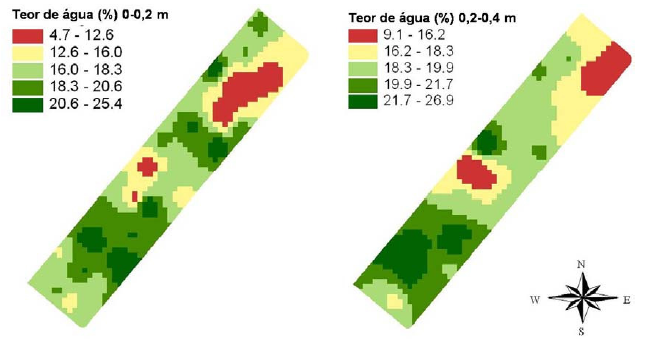
\includegraphics[width=10cm,angle=0]{imagens/grafico_1}
\caption{Mapas de teor de água das camadas de 0-2,2 e 0,2-0,4 m de profundidade.}
\label{fig:nome_referencia_figura1}
\end{figure}

\begin{figure}[ht]
\centering
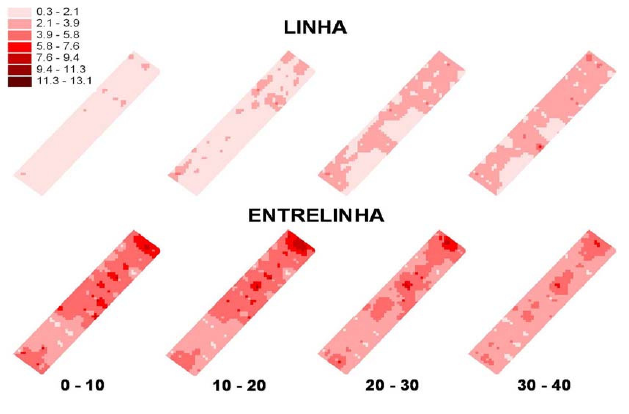
\includegraphics[width=10cm,angle=0]{imagens/grafico_2.png}
\caption{Mapas do índice de cone (MPa) referente aos dados coletados nas diferentes profundidades nas linhas e nas entrelinhas da cultura da cana.}
\label{fig:nome_referencia_figura2}
\end{figure}

\newpage
\noindent\textbf{Modelo de Tabela:}

\begin{table}[ht]
\caption{Análise do IC nas linhas (L) e entrelinhas (E) de cana nas diferentes profundidades amostradas pelo índice de cone.}
\vspace{.2cm}
\centering
\resizebox{\textwidth}{!}{%
\begin{tabular}{ccccccccc}
\hline
Profundidade (m) & \multicolumn{2}{c}{0 a 0,1} & \multicolumn{2}{c}{0,1 a 0,2} & \multicolumn{2}{c}{0,2 a 0,3} & \multicolumn{2}{c}{0,3 a 0,4} \\ \hline
                 & L            & E            & L             & E             & L             & E             & L             & E             \\
Média (MPa)      & 1,39**       & 4,28**       & 1,86**        & 4,29**        & 2,20**        & 3,83**        & 2,46**        & 3,44**        \\
CV(\%)           & 54           & 57           & 55            & 54            & 46            & 49            & 48            & 43            \\ \hline
\end{tabular}%
}
\small{**:valores significativos para o nível de significância de 1\% pelo teste de Tukey; L – linhas; E – entrelinhas.}
\label{tab:nome_tabela1}
\end{table} %Resultados e Discussão

\section*{Conclusões}

Devem basear-se exclusivamente nos resultados do trabalho. Evitar a repetição dos resultados em listagem subsequente, buscando, sim, confrontar o que se obteve com os objetivos inicialmente estabelecidos.

\section*{CONTRIBUIÇÕES DOS AUTORES}
Apresente de forma simplificada as contribuições de cada autor. Esta seção é baseada na Taxonomia CRediT e visa descrever as contribuições dos autores no trabalho. Como sugestão, utilize o Guia para Marcação e Publicação de contribuição de autores: Taxonomia CRediT da Scielo, disponível em: \url{https://wp.scielo.org/wp-content/uploads/credit.pdf}.

Exemplo: M.F.C, E.B.M.S e K.L.G. (podem ser utilizadas as iniciais do nome) contribuíram com a concepção e escopo do estudo. H.F.S e M.F.C procederam com a metodologia e experimentos. M.S.L, K.L.G. e E.B.M.S escreveram o trabalho.

Todos os autores contribuíram com a revisão do trabalho e aprovaram a versão submetida.


\section*{Agradecimentos}

Inserir após as conclusões, de maneira sucinta. Se o projeto for financiado por alguma agência de fomento, citar a fonte. %Conclusão, Contribuição e Agradecimentos


%Referências Bibliográficas
%\textbf{REFERÊNCIAS}

\bibliography{bibliografia.bib}
%\printbibliography[title={REFERÊNCIAS}]
%\printbibliography{bibliografia}



\end{document}